%╔════════════════════════════╗
%║	  Szablon dostosował	  ║
%║	mgr inż. Dawid Kotlarski  ║
%║		  06.10.2024		  ║
%╚════════════════════════════╝


\documentclass[12pt,twoside,a4paper,openany]{article}

    % ------------------------------------------------------------------------
% PAKIETY
% ------------------------------------------------------------------------

%różne pakiety matematyczne, warto przejrzeć dokumentację, muszą być powyżej ustawień językowych.
\usepackage{mathrsfs}   %Różne symbole matematyczne opisane w katalogu ~\doc\latex\comprehensive. Zamienia \mathcal{L} ze zwykłego L na L-transformatę.
\usepackage{eucal}      %Różne symbole matematyczne.
\usepackage{amssymb}    %Różne symbole matematyczne.
\usepackage{amsmath}    %Dodatkowe funkcje matematyczne, np. polecenie \dfac{}{} skladajace ulamek w trybie wystawionym (porównaj $\dfrac{1}{2}$, a $\frac{1}{2}$).

%język polski i klawiatura
\usepackage[polish]{babel}
\usepackage{csquotes}
%\usepackage{qtimes} % czcionka Times new Roman
\usepackage{polski}

\usepackage{ifluatex}

\ifluatex
  %czcionka
  \usepackage{fontspec}
  \setmainfont{Calibri}

  %obsługa pdf'a
  \usepackage[luatex,usenames,dvipsnames]{color}      %Obsługa kolorów. Opcje usenames i dvipsnames wprowadzają dodatkowe nazwy kolorow.
  \usepackage[luatex,pagebackref=false,draft=false,pdfpagelabels=false,colorlinks=true,urlcolor=cyan,linkcolor=blue,filecolor=magenta,citecolor=green,pdfstartview=FitH,pdfstartpage=1,pdfpagemode=UseOutlines,bookmarks=true,bookmarksopen=true,bookmarksopenlevel=2,bookmarksnumbered=true,pdfauthor={Dawid Kotlarski},pdftitle={Dokumentacja Projektowa},pdfsubject={},pdfkeywords={transient recovery voltage trv},unicode=true]{hyperref}   %Opcja pagebackref=true dotyczy bibliografii: pokazuje w spisie literatury numery stron, na których odwołano się do danej pozycji.
\else
  \usepackage[pdftex,usenames,dvipsnames]{color}      %Obsługa kolorów. Opcje usenames i dvipsnames wprowadzają dodatkowe nazwy kolorow.
\usepackage[pdftex,pagebackref=false,draft=false,pdfpagelabels=false,colorlinks=true,urlcolor=blue,linkcolor=black,citecolor=green,pdfstartview=FitH,pdfstartpage=1,pdfpagemode=UseOutlines,bookmarks=true,bookmarksopen=true,bookmarksopenlevel=2,bookmarksnumbered=true,pdfauthor={Dawid Kotlarski},pdftitle={Dokumentacja Projektowa},pdfsubject={},pdfkeywords={transient recovery voltage trv},unicode=true]{hyperref}  %Opcja pagebackref=true dotyczy bibliografii: pokazuje w spisie literatury numery stron, na których odwołano się do danej pozycji.
\fi

%bibliografia
%\usepackage[numbers,sort&compress]{natbib}  %Porządkuje zawartość odnośników do literatury, np. [2-4,6]. Musi być pod pdf'em, a styl bibliogfafii musi mieć nazwę z dodatkiem 'nat', np. \bibliographystyle{unsrtnat} (w kolejności cytowania).
\usepackage[
  backend=biber,
  style=numeric,
  sorting=none
]{biblatex}
\addbibresource{bibliografia.bib}
\usepackage{hypernat}                       %Potrzebna pakietowi natbib do wspolpracy z pakietem hyperref (wazna kolejnosc: 1. hyperref, 2. natbib, 3. hypernat).

%grafika i geometria strony
\usepackage{extsizes}           %Dostepne inne rozmiary czcionek, np. 14 w poleceniu: \documentclass[14pt]{article}.
\usepackage[final]{graphicx}
\usepackage[a4paper,left=1.5cm,right=1.5cm,top=2.5cm,bottom=2.5cm]{geometry}

%strona tytułowa
\usepackage{strona_tytulowa}

%inne
\usepackage{lastpage} %! do numerowania stron w formacie (x z y)
\usepackage[hide]{todo}                     %Wprowadza polecenie \todo{treść}. Opcje pakietu: hide/show. Polecenie \todos ma byc na koncu dokumentu, wszystkie \todo{} po \todos sa ignorowane.
\usepackage[basic,physics]{circ}            %Wprowadza środowisko circuit do rysowania obwodów elektrycznych. Musi byc poniżej pakietow językowych.
\usepackage[sf,bf,outermarks]{titlesec}     %Troszczy się o wygląd tytułów rozdziałów (section, subsection, ...). sf oznacza czcionkę sans serif (typu arial), bf -- bold. U mnie: oddzielna linia dla naglowku paragraph. Patrz tez: tocloft -- lepiej robi format spisu tresci.
\usepackage{tocloft}                        %Troszczy się o format spisu trsci.
\usepackage{expdlist}    %Zmienia definicję środowiska description, daje większe możliwości wpływu na wygląd listy.
\usepackage{flafter}     %Wprowadza parametr [tb] do polecenia \suppressfloats[t] (polecenie to powoduje nie umieszczanie rysunkow, tabel itp. na stronach, na ktorych jest to polecenie (np. moze byc to stroma z tytulem rozdzialu, ktory chcemy zeby byl u samej gory, a nie np. pod rysunkiem)).
\usepackage{array}       %Ładniej drukuje tabelki (np. daje wiecej miejsca w komorkach -- nie są tak ścieśnione, jak bez tego pakietu).
\usepackage{listings}    %Listingi programow.
\usepackage[format=hang,labelsep=period,labelfont={bf,small},textfont=small]{caption}   %Formatuje podpisy pod rysunkami i tabelami. Parametr 'hang' powoduje wcięcie kolejnych linii podpisu na szerokosc nazwy podpisu, np. 'Rysunek 1.'.
\usepackage{appendix}    %Troszczy się o załączniki.
\usepackage{floatflt}    %Troszczy się o oblewanie rysunkow tekstem.
\usepackage{here}        %Wprowadza dodtkowy parametr umiejscowienia rysunków, tabel, itp.: H (duże). Umiejscawia obiekty ruchome dokladnie tam gdzie są w kodzie źródłowym dokumentu.
\usepackage{makeidx}     %Troszczy się o indeks (skorowidz).

%nieużywane, ale potencjalnie przydatne
\usepackage{sectsty}           %Formatuje nagłówki, np. żeby były kolorowe -- polecenie: \allsectionsfont{\color{Blue}}.
%\usepackage{version}           %Wersje dokumentu.

%============
\usepackage{longtable}			%tabelka
\usepackage{tabularx}
%============

%============
% Ustawienia listingów do kodu
%============

\usepackage{listings}
\usepackage{xcolor}

\usepackage{hyperref}
\usepackage{booktabs}

\definecolor{codegreen}{rgb}{0,0.6,0}
\definecolor{codegray}{rgb}{0.5,0.5,0.5}
\definecolor{codepurple}{rgb}{0.58,0,0.82}
\definecolor{backcolour}{rgb}{0.95,0.95,0.92}

% Definicja stylu "mystyle"
\lstdefinestyle{mystyle}{
backgroundcolor=\color{backcolour},
commentstyle=\color{codegreen},
keywordstyle=\color{blue},	%magenta
numberstyle=\tiny\color{codegray},
stringstyle=\color{codepurple},
basicstyle=\ttfamily\footnotesize,
breakatwhitespace=false,
breaklines=true,
captionpos=b,
keepspaces=true,
numbers=left,
numbersep=5pt,
showspaces=false,
showstringspaces=false,
showtabs=false,
tabsize=2,
literate=
  {á}{{\'a}}1 {é}{{\'e}}1 {í}{{\'i}}1 {ó}{{\'o}}1 {ú}{{\'u}}1
{Á}{{\'A}}1 {É}{{\'E}}1 {Í}{{\'I}}1 {Ó}{{\'O}}1 {Ú}{{\'U}}1
{à}{{\`a}}1 {è}{{\`e}}1 {ì}{{\`i}}1 {ò}{{\`o}}1 {ù}{{\`u}}1
{À}{{\`A}}1 {È}{{\`E}}1 {Ì}{{\`I}}1 {Ò}{{\`O}}1 {Ù}{{\`U}}1
{ä}{{\"a}}1 {ë}{{\"e}}1 {ï}{{\"i}}1 {ö}{{\"o}}1 {ü}{{\"u}}1
{Ä}{{\"A}}1 {Ë}{{\"E}}1 {Ï}{{\"I}}1 {Ö}{{\"O}}1 {Ü}{{\"U}}1
{â}{{\^a}}1 {ê}{{\^e}}1 {î}{{\^i}}1 {ô}{{\^o}}1 {û}{{\^u}}1
{Â}{{\^A}}1 {Ê}{{\^E}}1 {Î}{{\^I}}1 {Ô}{{\^O}}1 {Û}{{\^U}}1
{ã}{{\~a}}1 {ẽ}{{\~e}}1 {ĩ}{{\~i}}1 {õ}{{\~o}}1 {ũ}{{\~u}}1
{Ã}{{\~A}}1 {Ẽ}{{\~E}}1 {Ĩ}{{\~I}}1 {Õ}{{\~O}}1 {Ũ}{{\~U}}1
{œ}{{\oe}}1 {Œ}{{\OE}}1 {æ}{{\ae}}1 {Æ}{{\AE}}1 {ß}{{\ss}}1
{ű}{{\H{u}}}1 {Ű}{{\H{U}}}1 {ő}{{\H{o}}}1 {Ő}{{\H{O}}}1
{ç}{{\c c}}1 {Ç}{{\c C}}1 {ø}{{\o}}1 {Ø}{{\O}}1 {å}{{\r a}}1 {Å}{{\r A}}1
{€}{{\euro}}1 {£}{{\pounds}}1 {«}{{\guillemotleft}}1
{»}{{\guillemotright}}1 {ñ}{{\~n}}1 {Ñ}{{\~N}}1 {¿}{{?`}}1 {¡}{{!`}}1
{ą}{{\k{a}}}1 {ć}{{\'{c}}}1 {ę}{{\k{e}}}1 {ł}{{\l}}1 {ń}{{\'n}}1
{ó}{{\'o}}1 {ś}{{\'s}}1 {ź}{{\'z}}1 {ż}{{\.{z}}}1
{Ą}{{\k{A}}}1 {Ć}{{\'{C}}}1 {Ę}{{\k{E}}}1 {Ł}{{\L}}1 {Ń}{{\'N}}1
{Ó}{{\'O}}1 {Ś}{{\'S}}1 {Ź}{{\'Z}}1 {Ż}{{\.{Z}}}1
}

\lstset{style=mystyle} % Deklaracja aktywnego stylu
%===========

%PAGINA GÓRNA I DOLNA
\usepackage{fancyhdr}          %Dodaje naglowki jakie się chce.
\pagestyle{fancy}
\fancyhf{}
% numery stron na środku dolnej stopki
\fancyfoot[C]{\footnotesize DOKUMENTACJA PROJEKTOWA – SYSTEMY OPERACYJNE  \\
  \normalsize\sffamily  \thepage\ z~\pageref{LastPage}}

%\fancyhead[L]{\small\sffamily \nouppercase{\leftmark}}
\fancyhead[C]{\footnotesize \textit{AKADEMIA NAUK STOSOWANYCH W NOWYM SĄCZU}\\}

\renewcommand{\headrulewidth}{0.4pt}
\renewcommand{\footrulewidth}{0.4pt}

    % ------------------------------------------------------------------------
% USTAWIENIA
% ------------------------------------------------------------------------

% ------------------------------------------------------------------------
%   Kropki po numerach sekcji, podsekcji, itd.
%   Np. 1.2. Tytuł podrozdziału
% ------------------------------------------------------------------------
\makeatletter
    \def\numberline#1{\hb@xt@\@tempdima{#1.\hfil}}                      %kropki w spisie treści
    \renewcommand*\@seccntformat[1]{\csname the#1\endcsname.\enspace}   %kropki w treści dokumentu
\makeatother

% ------------------------------------------------------------------------
%   Numeracja równań, rysunków i tabel
%   Np.: (1.2), gdzie:
%   1 - numer sekcji, 2 - numer równania, rysunku, tabeli
%   Uwaga ogólna: o otoczeniu figure ma być najpierw \caption{}, potem \label{}, inaczej odnośnik nie działa!
% ------------------------------------------------------------------------
\makeatletter
    \@addtoreset{equation}{section} %resetuje licznik po rozpoczęciu nowej sekcji
    \renewcommand{\theequation}{{\thesection}.\@arabic\c@equation} %dodaje kropki

    \@addtoreset{figure}{section}
    \renewcommand{\thefigure}{{\thesection}.\@arabic\c@figure}

    \@addtoreset{table}{section}
    \renewcommand{\thetable}{{\thesection}.\@arabic\c@table}
\makeatother

% ------------------------------------------------------------------------
% Tablica
% ------------------------------------------------------------------------
\newenvironment{tabela}[3]
{
    \begin{table}[!htb]
    \centering
    \caption[#1]{#2}
    \vskip 9pt
    #3
}{
    \end{table}
}

% ------------------------------------------------------------------------
% Dostosowanie wyglądu pozycji listy \todos, np. zamiast 'p.' jest 'str.'
% ------------------------------------------------------------------------
\renewcommand{\todoitem}[2]{%
    \item \label{todo:\thetodo}%
    \ifx#1\todomark%
        \else\textbf{#1 }%
    \fi%
    (str.~\pageref{todopage:\thetodo})\ #2}
\renewcommand{\todoname}{Do zrobienia...}
\renewcommand{\todomark}{~uzupełnić}

% ------------------------------------------------------------------------
% Definicje
% ------------------------------------------------------------------------
\def\nonumsection#1{%
    \section*{#1}%
    \addcontentsline{toc}{section}{#1}%
    }
\def\nonumsubsection#1{%
    \subsection*{#1}%
    \addcontentsline{toc}{subsection}{#1}%
    }
\reversemarginpar %umieszcza notki po lewej stronie, czyli tam gdzie jest więcej miejsca
\def\notka#1{%
    \marginpar{\footnotesize{#1}}%
    }
\def\mathcal#1{%
    \mathscr{#1}%
    }
\newcommand{\atp}{ATP/EMTP} % Inaczej: \def\atp{ATP/EMTP}

% ------------------------------------------------------------------------
% Inne
% ------------------------------------------------------------------------
\frenchspacing                      
\hyphenation{ATP/-EMTP}             %dzielenie wyrazu w danym miejscu
\setlength{\parskip}{3pt}           %odstęp pomiędzy akapitami
\linespread{1.3}                    %odstęp pomiędzy liniami (interlinia)
\setlength{\headheight}{22.48892pt} %ustawienie wysokości nagłówka
\addtolength{\topmargin}{-10.48892pt} %dostosowanie górnego marginesu
\setcounter{tocdepth}{4}            %uwzględnianie w spisie treści czterech poziomów sekcji
\setcounter{secnumdepth}{4}         %numerowanie do czwartego poziomu sekcji 
\titleformat{\paragraph}[hang]      %wygląd nagłówków
{\normalfont\sffamily\bfseries}{\theparagraph}{1em}{}

%komenda do łatwiejszego wstawiania zdjęć
\newcommand*{\fg}[4][\textwidth]{
    \begin{figure}[!htb]
        \begin{center}
            \includegraphics[width=#1]{#2}
            \caption{#3}
            \label{rys:#4}
        \end{center}
    \end{figure}
}

\newcommand*{\Oznacz}[2]{
\ref{#1:#2} (s. \pageref{#1:#2})
}

\newcommand*{\OznaczZdjecie}[2][Rysunek]{
#1 \Oznacz{rys}{#2}
}
    
\newcommand*{\OznaczKod}[1]{
\Oznacz{lst}{#1}
}

\newcommand*{\ListingFile}[2]{
    \lstinputlisting[caption=#1, label={lst:#2}, language=C++]{kod/#2.txt}
}


    %polecenia zdefiniowane w pakiecie strona_tytulowa.sty
    \title{Konfiguracja Site-to-Site VPN w Cisco IOS}		%...Wpisać nazwę projektu...
    \author{Imie Nazwisko}
    \author{Arkadiusz Ryczek, Maciej Wójs,  }
    \authorI{Dominik Żuchowicz, Hubert Zięba}
    \authorII{Szymon Wolski, Filip Wąchała, Jakub \textit{Józef} Tokarczyk}		%jeśli są dwie osoby w projekcie to zostawiamy:    \authorII{}
		
	\uczelnia{AKADEMIA NAUK STOSOWANYCH \\W NOWYM SĄCZU}
    \instytut{Wydział Nauk Inżynieryjnych}
    \kierunek{Katedra Informatyki}
    \praca{DOKUMENTACJA PROJEKTOWA}
    \przedmiot{BEZPIECZEŃSTWO SYSTEMÓW INFORMATYCZNYCH}
    \prowadzacy{mgr inż. Jacek Kaleta}
    \rok{2025}

    \definecolor{codegreen}{rgb}{0,0.6,0}
    \definecolor{codegray}{rgb}{0.5,0.5,0.5}
    \definecolor{codepurple}{rgb}{0.58,0,0.82}
    \definecolor{backcolour}{rgb}{0.95,0.95,0.92}

    \lstdefinestyle{mystyle}{
        backgroundcolor=\color{backcolour},   
        commentstyle=\color{codegreen},
        keywordstyle=\color{magenta},
        numberstyle=\tiny\color{codegray},
        stringstyle=\color{codepurple},
        basicstyle=\ttfamily\footnotesize,
        breakatwhitespace=false,         
        breaklines=true,                 
        captionpos=b,                    
        keepspaces=true,                 
        numbers=left,                    
        numbersep=5pt,                  
        showspaces=false,                
        showstringspaces=false,
        showtabs=false,                  
        tabsize=2,
        morecomment=[l]{!}
    }

    \lstset{style=mystyle}
%definicja składni mikrotik
\usepackage{fancyvrb}
\DefineVerbatimEnvironment{MT}{Verbatim}%
{commandchars=\+\[\],fontsize=\small,formatcom=\color{red},frame=lines,baselinestretch=1,} 
\let\mt\verb
%zakonczenie definicji składni mikrotik

\usepackage{fancyhdr}    %biblioteka do nagłówka i stopki
\begin{document}

\renewcommand{\figurename}{Rys.}    %musi byc pod \begin{document}, bo w~tym miejscu pakiet 'babel' narzuca swoje ustawienia
\renewcommand{\tablename}{Tab.}     %j.w.
\thispagestyle{empty}               %na tej stronie: brak numeru
\stronatytulowa                     %strona tytułowa tworzona przez pakiet strona_tytulowa.tex

% \input{tabela.tex} % tabela z danymi projektu

\pagestyle{fancy}
\newpage

%formatowanie spisu treści i~nagłówków
\renewcommand{\cftbeforesecskip}{8pt}
\renewcommand{\cftsecafterpnum}{\vskip 8pt}
\renewcommand{\cftparskip}{3pt}
\renewcommand{\cfttoctitlefont}{\Large\bfseries\sffamily}
\renewcommand{\cftsecfont}{\bfseries\sffamily}
\renewcommand{\cftsubsecfont}{\sffamily}
\renewcommand{\cftsubsubsecfont}{\sffamily}
\renewcommand{\cftparafont}{\sffamily}
%koniec formatowania spisu treści i nagłówków

\tableofcontents    %spis treści
\thispagestyle{fancy}
\newpage

%%%%%%%%%%%%%%%%%%% treść główna dokumentu %%%%%%%%%%%%%%%%%%%%%%%%%
\section{Wymagania projektu}
\begin{itemize}
\item \textbf{Topologia:} Dwa oddzielne lokacje (Site A i Site B) połączone przez publiczną sieć ISP
\item \textbf{Urządzenia:} Dwa routery Cisco (R1 i R3) pełniące rolę bram VPN
\item \textbf{Wymagania bezpieczeństwa:}
  \begin{itemize}
  \item Szyfrowanie ruchu między lokacjami
  \item Uwierzytelnianie urządzeń
  \item Integralność przesyłanych danych
  \end{itemize}
\item \textbf{Wymagania funkcjonalne:}
  \begin{itemize}
  \item Tunel IPSec między R1 (10.1.1.1) i R3 (10.2.2.1)
  \item Komunikacja między sieciami LAN (192.168.1.0/24 i 192.168.3.0/24)
  \item Wykorzystanie pre-shared key do uwierzytelniania
  \end{itemize}
\end{itemize}

\section{Topologia sieci}
\begin{figure}[h!]
\centering
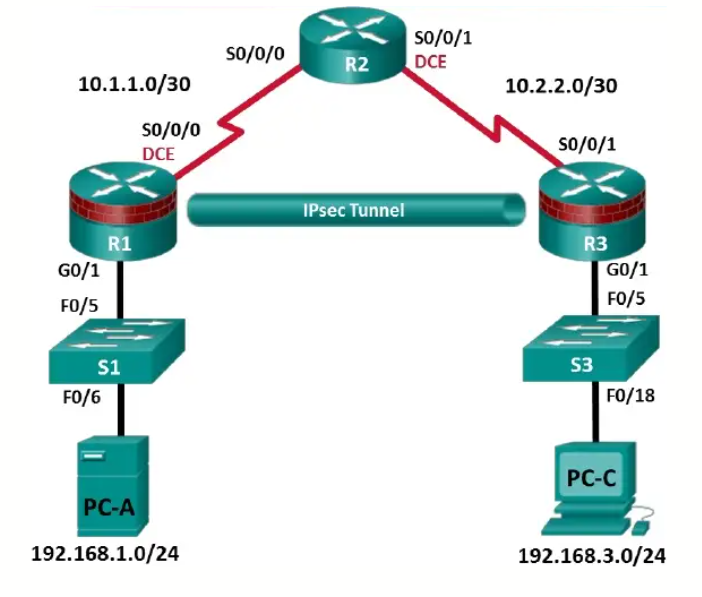
\includegraphics[width=0.8\textwidth]{rys/Screenshot From 2025-06-09 18-29-04.png}
\caption{Topologia połączenia VPN między Site A i Site B}
\label{fig:vpn_topology}
\end{figure}
\textbf{Uwaga:} Router R2 pełni rolę symulowanego dostawcy internetowego (ISP) i nie uczestniczy w konfiguracji VPN.

\section{Tabela adresacji IP}
\begin{figure}[h!]
    \centering
    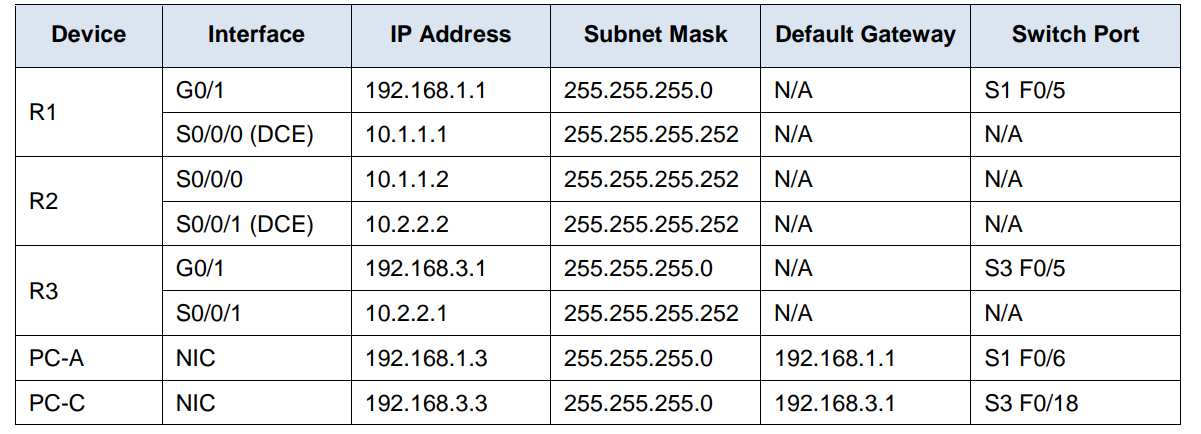
\includegraphics[width=0.95\textwidth]{rys/adresy.png}
    \caption{Tabela adresacji IP dla urządzeń w projekcie}
    \label{fig:adresacja_ip}
\end{figure}

\section{Konfiguracja routera R1}
\begin{lstlisting}[caption={Konfiguracja podstawowa i VPN na R1}]
! Konfiguracja interfejsów
! Przypisanie adresu IP do interfejsu GigabitEthernet0/1 (sieć LAN Site A)
interface GigabitEthernet0/1
 ip address 192.168.1.1 255.255.255.0
 no shutdown! Aktywacja interfejsu
!
! Przypisanie adresu IP do interfejsu Serial0/0/0 (połączenie z ISP)
interface Serial0/0/0
 ip address 10.1.1.1 255.255.255.252
 no shutdown! Aktywacja interfejsu

! Routing statyczny
! Definicja trasy domyślnej kierującej ruch do ISP
ip route 0.0.0.0 0.0.0.0 10.1.1.2

! Konfiguracja ISAKMP (IKE Phase 1)
! Definicja polityki ISAKMP (Internet Security Association and Key Management Protocol)
crypto isakmp policy 10
 encr 3des            !Użycie szyfrowania 3DES
 hash md5             !Użycie funkcji skrótu MD5
 authentication pre-share !Metoda uwierzytelniania: pre-shared key
 group 2              !Grupa Diffie-Hellmana (DH) numer 2 (1024-bit)
! Definicja klucza pre-shared dla zdalnego routera (R3)
crypto isakmp key cisco123 address 10.2.2.1

! Konfiguracja transform set (IKE Phase 2)
! Definicja zestawu transformacji określającego, jak dane będą chronione
crypto ipsec transform-set MYSET esp-3des esp-md5-hmac
! esp-3des: Szyfrowanie ESP (Encapsulating Security Payload) za pomocą 3DES
! esp-md5-hmac: Uwierzytelnianie ESP za pomocą HMAC-MD5

! Definicja listy dostępu dla ruchu VPN
! Określenie, który ruch sieciowy ma być szyfrowany (z LAN Site A do LAN Site B)
ip access-list extended VPN-TRAFFIC
 permit ip 192.168.1.0 0.0.0.255 192.168.3.0 0.0.0.255

! Tworzenie i aplikacja mapy kryptograficznej
! Powiązanie wszystkich elementów konfiguracji VPN w jedną całość
crypto map MYMAP 10 ipsec-isakmp
 set peer 10.2.2.1            !Adres IP zdalnego routera VPN (R3)
 set transform-set MYSET      !Użycie zdefiniowanego zestawu transformacji
 match address VPN-TRAFFIC    !Powiązanie z listą dostępu definiującą ruch VPN

! Aplikacja mapy kryptograficznej do interfejsu wychodzącego (w kierunku ISP)
interface Serial0/0/0
 crypto map MYMAP
\end{lstlisting}

\section{Konfiguracja routera R3}
\begin{lstlisting}[caption={Konfiguracja podstawowa i VPN na R3}]
! Konfiguracja interfejsów
! Przypisanie adresu IP do interfejsu GigabitEthernet0/1 (sieć LAN Site B)
interface GigabitEthernet0/1
 ip address 192.168.3.1 255.255.255.0
 no shutdown! Aktywacja interfejsu
!
! Przypisanie adresu IP do interfejsu Serial0/0/1 (połączenie z ISP)
interface Serial0/0/1
 ip address 10.2.2.1 255.255.255.252
 no shutdown! Aktywacja interfejsu

! Routing statyczny
! Definicja trasy domyślnej kierującej ruch do ISP
ip route 0.0.0.0 0.0.0.0 10.2.2.2

! Konfiguracja ISAKMP (IKE Phase 1)
! Definicja polityki ISAKMP, musi być zgodna z konfiguracją na R1
crypto isakmp policy 10
 encr 3des
 hash md5
 authentication pre-share
 group 2
! Definicja klucza pre-shared dla zdalnego routera (R1)
crypto isakmp key cisco123 address 10.1.1.1

! Konfiguracja transform set (IKE Phase 2)
! Definicja zestawu transformacji, musi być zgodna z konfiguracją na R1
crypto ipsec transform-set MYSET esp-3des esp-md5-hmac

! Definicja listy dostępu dla ruchu VPN
! Określenie, który ruch sieciowy ma być szyfrowany (z LAN Site B do LAN Site A)
ip access-list extended VPN-TRAFFIC
 permit ip 192.168.3.0 0.0.0.255 192.168.1.0 0.0.0.255

! Tworzenie i aplikacja mapy kryptograficznej
! Powiązanie wszystkich elementów konfiguracji VPN w jedną całość
crypto map MYMAP 10 ipsec-isakmp
 set peer 10.1.1.1            !Adres IP zdalnego routera VPN (R1)
 set transform-set MYSET      !Użycie zdefiniowanego zestawu transformacji
 match address VPN-TRAFFIC    !Powiązanie z listą dostępu definiującą ruch VPN

! Aplikacja mapy kryptograficznej do interfejsu wychodzącego (w kierunku ISP)
interface Serial0/0/1
 crypto map MYMAP
\end{lstlisting}

% \section{Weryfikacja działania VPN}
% \subsection{Polecenia weryfikacyjne}
% \begin{lstlisting}
% show crypto isakmp sa      # Wyświetla status skojarzeń bezpieczeństwa IKE (Phase 1)
% show crypto ipsec sa       # Wyświetla status tuneli IPSec (Phase 2) i statystyki ruchu
% ping 192.168.3.10 source 192.168.1.10  # Testuje połączenie end-to-end przez tunel VPN
%                                        # (przy założeniu, że hosty istnieją w obu sieciach)
% \end{lstlisting}

% \subsection{Oczekiwane wyniki}
% \begin{itemize}
% \item Status IKE: \texttt{QM\_IDLE} oznacza poprawnie nawiązane sąsiedztwo
% \item Status IPSec: \texttt{\#pkts encaps/decaps} pokazuje przepływ ruchu
% \item Udany ping między sieciami lokalnymi
% \end{itemize}

% \section{Opis kluczowych parametrów}
% \begin{tabularx}{\textwidth}{lX} % Usunięto pionowe linie
% \toprule % Zamiast \hline
% \textbf{Parametr} & \textbf{Znaczenie} \\
% \midrule % Zamiast \hline
% ISAKMP Policy 10 & Definicja parametrów IKE Phase 1 \\
% esp-3des & Szyfrowanie 3DES (168-bit) \\
% esp-md5-hmac & Algorytm integralności MD5 \\
% pre-share & Uwierzytelnianie za pomocą wspólnego klucza \\
% group 2 & Grupa Diffie-Hellman 1024-bit \\
% crypto map & Mapowanie polityk bezpieczeństwa na interfejs \\
% match address & Powiązanie ACL z mapą kryptograficzną \\
% \bottomrule % Zamiast \hline
% \end{tabularx}
\clearpage
\section{Zrzuty ekranu}

\begin{figure}[h!]
    \centering
    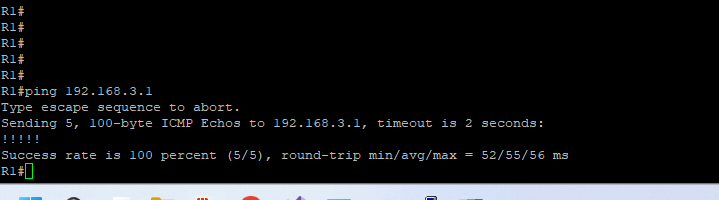
\includegraphics[width=0.75\textwidth]{routery/R1/ping1.png}
    \caption{Ping z R1 cz.1}
    \label{fig:adresacja_ip}
\end{figure}

\begin{figure}[ht!]
    \centering
    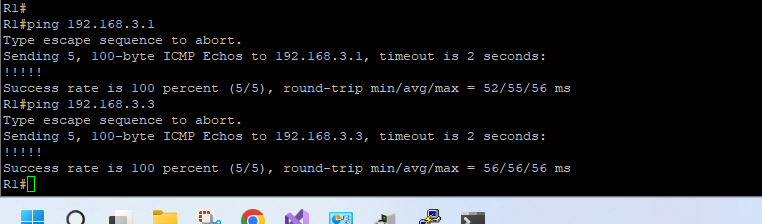
\includegraphics[width=0.75\textwidth]{routery/R1/ping2.png}
    \caption{Ping z R1 cz.2}
    \label{fig:adresacja_ip}
\end{figure}

\begin{figure}[ht!]
    \centering
    \begin{minipage}[t]{0.48\textwidth}
        \centering
        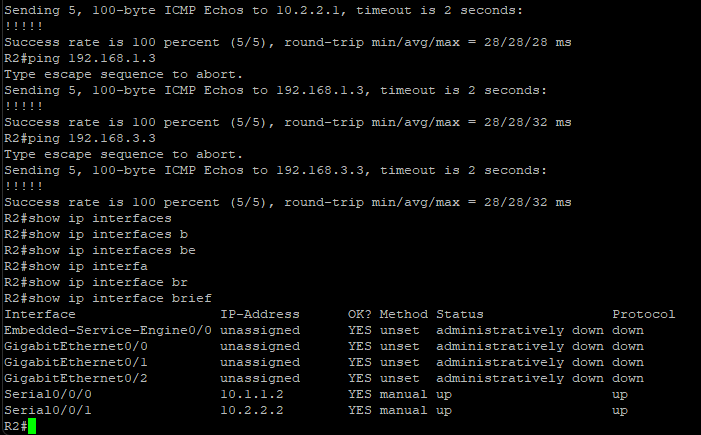
\includegraphics[width=\textwidth]{routery/R2/R2.png}
        \caption{Pingi do R2 oraz interfejsy}
        \label{fig:r2_ping}
    \end{minipage}
    \hfill
    \begin{minipage}[t]{0.48\textwidth}
        \centering
        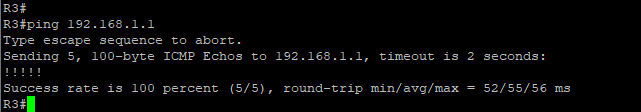
\includegraphics[width=\textwidth]{routery/R3/Zrzut ekranu 2025-06-02 194011.png}
        \caption{Pingi z R3 oraz interfejsy}
        \label{fig:r3_ping}
    \end{minipage}
\end{figure}
\clearpage
\section{Podsumowanie}
Konfiguracja Site-to-Site VPN obejmuje:
\begin{enumerate}
\item Konfigurację podstawową routerów (adresacja, routing)
\item Definicję polityki ISAKMP (IKE Phase 1)
\item Konfigurację transformacji IPSec (IKE Phase 2)
\item Tworzenie list dostępu identyfikujących ruch VPN
\item Budowę i aplikację map kryptograficznych
\end{enumerate}
Poprawnie skonfigurowany tunel VPN zapewnia bezpieczną komunikację między sieciami lokalnymi poprzez nieszyfrowaną sieć publiczną.
\end{document}
